\section{Game}
In this section we will discuss and explain our thoughts about the game design, we will also comment on the feedback given by our contact person. Finally we will show the result of the game design.
\subsection{Game Idea/Description}
%Skriv hvordan spillet fungere
In \secref{processweek2} it is explained how Tove's version of the exercise work. We intent keep the same principles of Tove's exercise. We will start by given a short description of the important objects of the game.
\begin{description}
\item[Pictogram] Is a object which contains a picture and is draggable.
\item[Train Station] Is a station where the train stops, and allows the child to drag and drop pictograms onto the station. Each station has a picture indicating the category of the station. The category of the station describes the pictograms that should be dropped onto the station.  

\item[Train whistle] Is a button that the child can press if they think that the correct pictograms have been dropped onto the station. If however the child have made a mistake and dropped a pictogram not belonging to the station's category, then the train will not start. The train whistle was added by Tove's request.

\item[Train and wagons] Is a vehicle that drives to each station, carrying pictograms in its wagons.

\item[Landscape] Is a sequence of hills, trees, cow, and skies. The landscape object is placed between each stations, and creates the illusion that the train is driving to the next station.

\item[Train depot] When the train is driving from the last train station, the train will drive into the a train depot to indicate the the game is over. The train depot was added by Tove's request.
\end{description}
Our game starts by the child must drag the pictograms off the start Train station and drop them onto the train, the start station is different since it does not have a category. The start station is to help the child understand how to move the pictograms with drag and drop. When the child has moved all the pictures onto the train, it is allowed to drive through a landscape object, until it reaches the first train station.
The Train station has a category, which could be a picture of animals. It is now up to the child to drag all the animals off the train onto the station, so the train can continue. If all the right pictograms is on the station, the train will drive onto the next station. When all the pictograms is off the train the game will end.

\subsection{Game Prototype}
%vis billedet af prototypen, beskriv hvad Tove godt kunne lide, og hvad der kunne ændres, samt tilføjelser. (fløjten, ingen musik, no fancy colors on objects)
\begin{figure}[H]
\centering
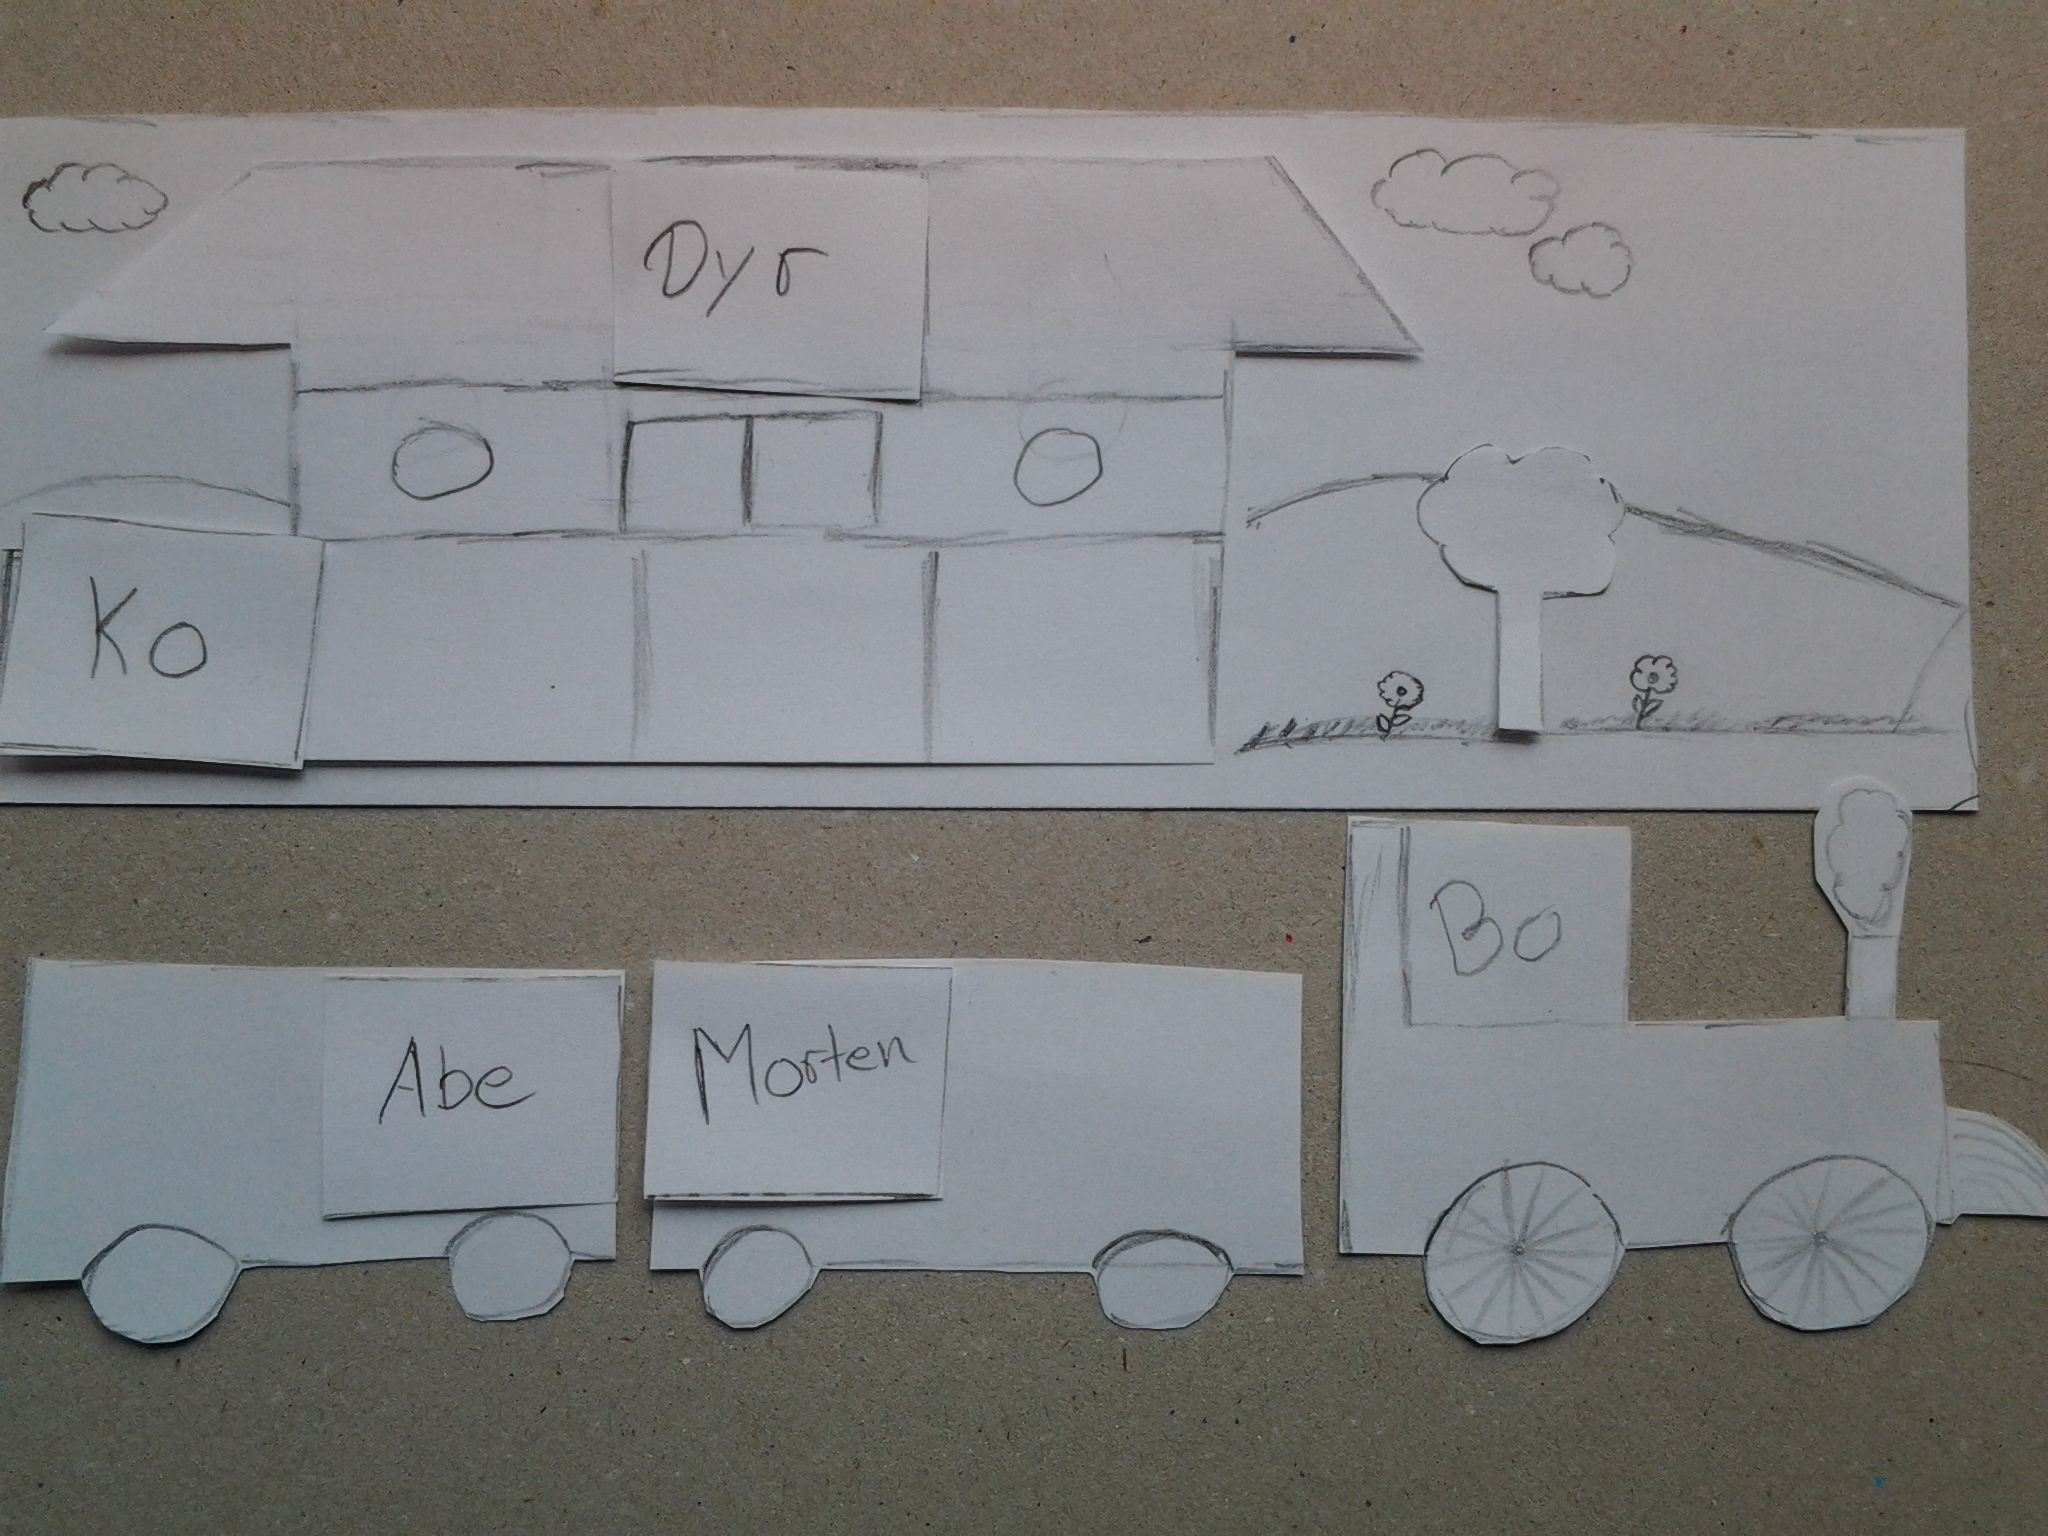
\includegraphics[width=0.9\linewidth]{img/screenshots/prototype1.jpg}%0.1 margin
\caption{The paper prototype}
\label{fig:paperprototype}
\end{figure}
\autoref{fig:paperprototype} shows the paper prototype we showed Tove at our first meeting, in which we explained our game idea. She liked the idea and the interface, although she would like to see a button that checks if the correct pictograms is off the train, if all pictograms is off, the train should start. She also mentioned that the game should have ending, she suggested that the train could drive into a train depot. The game should not contain many colors and sounds, since this would cause visual and audible noise for the child. The train whistle and train depot was added to the game idea after the meeting.


\subsection{Final Game Design}
\label{designgameinterface}
\todo{describe the final result, show off a station and the entire game with one station.}
During the project we sent screen shots of the game interface to Tove, to confirm that we were on the right track. For the most part she had not much to add, only small graphical adjustments to stations. 
In order to mimic Tove's version of the exercise we had to make the game customizable, we had to add a menu where Tove was able to customize the pictograms and the category for each station, the menu and its functionality is explained later in \secref{designmenu}. To prevent that the game is not the same every time we added random elements to the game, e.g. the order of stations, the hills in the landscape object, the decorative objects(cow, trees, skies) are all randomly placed. 
\begin{figure}[H]
\centering
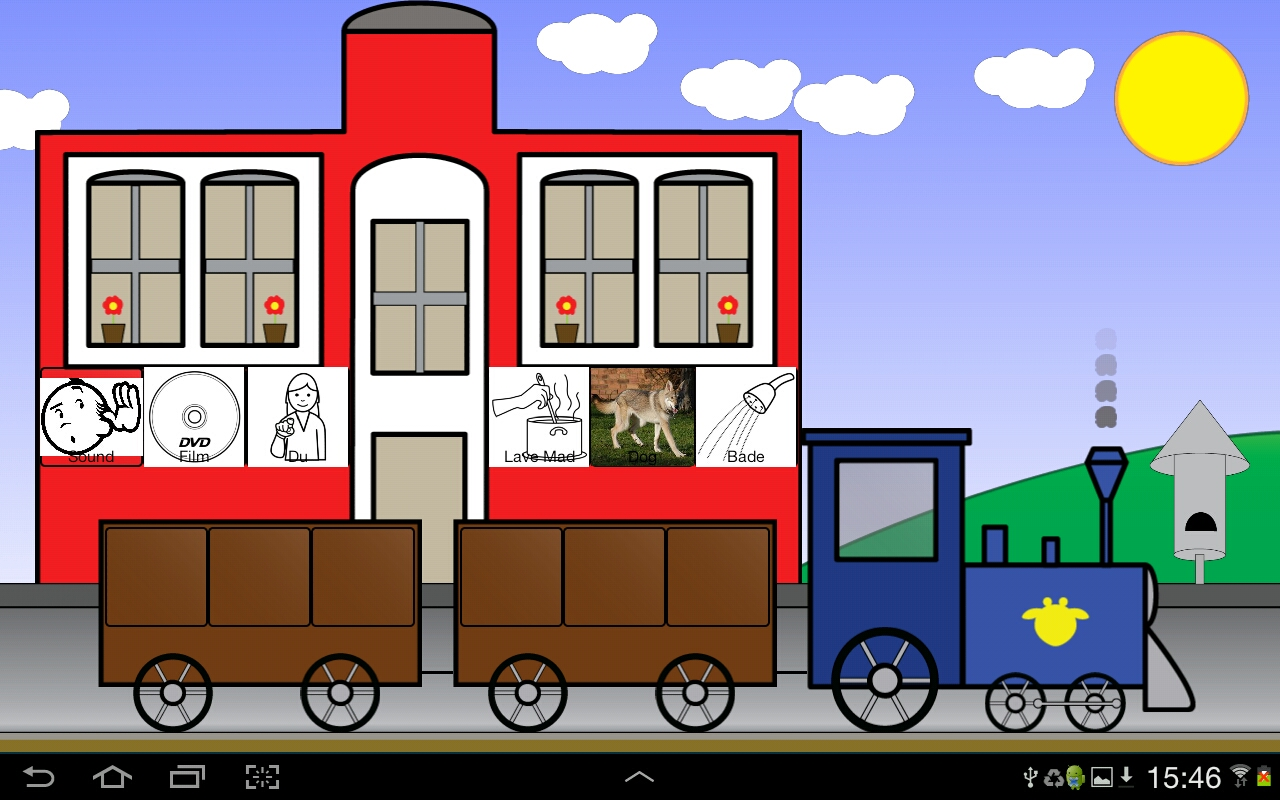
\includegraphics[width=0.9\linewidth]{img/screenshots/gamedesign1.jpg}%0.1 margin
\caption{The final result}
\label{fig:finalresult}
\end{figure}
\begin{figure}[H]
\centering
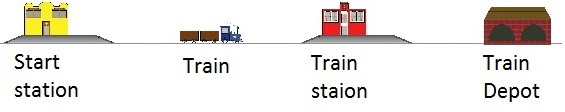
\includegraphics[width=0.9\linewidth]{img/screenshots/stations.jpg}%0.1 margin
\caption{Miniature game}
\label{fig:miniaturegame}
\end{figure}
\autoref{fig:finalresult} and \autoref{fig:miniaturegame} shows the final result of the game design. \todo{skriv lige hvad miniaturegame billedet viser}
%vis det endelig resultat, samt de ting som ikke noget at blive tilføjet.(Traindriver, click and autosnap, lyd på pictogrammer)
